\section{Free modules and vector spaces}
\begin{ex}
    \begin{enumerate}[(a)]
        \item A set of vectors $\{x_{1},\cdots x_{n}\}$ in a vector space $V$ over a division ring $R$ is linearly dependent if and only if some $x_{k}$ is a linear combination of the preceding $x_{i}$.
        \item If $\{x_{1},x_{2},x_{3}\}$ is a linearly independent subset of $V$, then the set $\{x_{1}+x_{2},x_{2}+x_{3},x_{3}+x_{1}\}$ is linearly independent if and only if $\mathrm{Char}R\neq 2$.
    \end{enumerate}
\end{ex}

\begin{answer}
    \begin{enumerate}[(a)]
        \item If $x_{k}$ is a linear combination of preceding $x_{i}$, then $x_{k}=r_{1}x_{1}+\cdots+r_{k-1}x_{k-1}+r_{k+1}x_{k+1}+\cdots+ r_{n}x_{n}$ with some $r_{i}\neq 0$, so $r_{1}x_{1}+\cdots+r_{k-1}x_{k-1}-x_{k}+r_{k+1}x_{k+1}+\cdots +r_{n}x_{n}=0$. So $\{x_{1},\cdots,x_{n}\}$ is linearly dependent.
        
        Conversely, $r_{1}x_{1}+\cdots+r_{n}x_{n}=0$ for some non-trivial $r_{i}$. WLOG, assume $r_{1}\neq 0$, then $x_{1}=(-\frac{r_{2}}{r_{1}})x_{2}+(-\frac{r_{3}}{r_{1}})x_{3}+\cdots+(-\frac{r_{n}}{r_{1}})x_{n}$ is a linear combination.
        \item If $\mathrm{char} R\neq 2$, $r_{1}(x_{1}+x_{2})+r_{2}(x_{2}+x_{3})+r_{3}(x_{1}+x_{3})=(r_{1}+r_{3})x_{1}+(r_{1}+r_{2})x_{2}+(r_{2}+r_{3})x_{3}=0$. $\{x_{1},x_{2},x_{3}\}$ is linearly independent, so $r_{1}+r_{3}=r_{1}+r_{2}=r_{2}+r_{3}=0$, $2r_{1}+r_{2}+r_{3}=2r_{1}=0$, we have $r_{1}=0$. Similarly, $r_{2}=r_{3}=0$, $\{x_{1}+x_{2},x_{2}+x_{3},x_{1}+x_{3}\}$ is linearly independent.
        
        Conversely, suppose $\mathrm{char}R=2$, $\exists r_{1},r_{2},r_{3}\in R$, $2r_{1}=2r_{2}=2r_{3}=0$. We have $(r_{1}+r_{2}-r_{3})(x_{1}+x_{2})+(r_{1}+r_{3}-r_{2})(x_{1}+x_{3})+(r_{3}+r_{2}-r_{1})(x_{3}+x_{2})=2r_{1}x_{1}+2r_{2}x_{2}+2r_{3}x_{3}=0$, but $r_{1}+r_{2}-r_{3}$, $r_{1}+r_{3}-r_{2}$, $r_{3}+r_{2}-r_{1}$ is not necessary to be 0.
    \end{enumerate}
\end{answer}

$$ $$

\begin{ex}
    Let $R$ be any ring (possibly without identity) and $X$ a nonempty set. In this exercise an $R$-module $F$ is called a \textbf{free module on $X$} if $F$ is a free object on $X$ in the category of all left $R$-modules. Thus by Definition I.7.7m $F$ is the free module on $X$ if there is a function $\tau:X\to F$ such that for any left $R$-module $A$ and function $f:X\to A$ there is a unique $R$-module homomorphism $\bar{f}:F\to A$ with $\bar{f}\tau=f$.
    \begin{enumerate}[(a)]
        \item Let $\{X_{i}|i\in I\}$ be a collection of mutually disjoint sets and for each $i\in I$, suppose $F_{i}$ is a free module on $X_{i}$, with $\tau_{i}:X_{i}\to F_{i}$. Let $X=\bigcup\limits_{i\in I}X_{i}$ and $F=\sum\limits_{i\in I}F_{i}$, with $\phi_{i}:F_{i}\to F$ the canonical injection. Define $\tau:X\to F$ by $\tau(x)=\phi_{i}\tau_{i}(x)$ for $x\in X_{i}$. Prove that $F$ is a free module on $X$.
        \item Assume $R$ has an identity. Let the abelian group $\mathbf{Z}$ be given trivial $R$-module structure ($rm=0$ for all $r\in R, m\in\mathbf{Z}$), so that $R\oplus\mathbf{Z}$ is an $R$-module with $r(r',m)=(rr',0)$ for all $r,r'\in R$, $m\in \mathbf{Z}$. If $X$ is any one element set, $X=\{t\}$, let $\tau:X\to R\oplus\mathbf{Z}$ be given by $\tau(t)=(1_{R},1)$. Prove that $R\oplus\mathbf{Z}$ is a free module on $X$.
        \item If $R$ is an arbitrary ring and $X$ is any set, then there exists a free module on $X$.
    \end{enumerate}
\end{ex}

\begin{answer}
    \begin{enumerate}[(a)]
        \item For any module $F'$ with $\tau':X\to F'$. For any $i\in I$, $\tau'|X_{i}:X_{i}\to F'$. Since $F$ is free on $X_{i}$, so there exists unique homomorphism $\psi_{i}:F_{i}\to F'$ s.t. $\tau'|X_{i}=\psi_{i}\tau_{i}$. $F$ is the coproduct of $F_{i}$, so there exists unique homomorphism $f:F\to F'$ s.t. $f\phi_{i}=\psi_{i}$. So $\tau'|X_{i}=f\phi_{i}\tau_{i}=f\tau$. $F$ is free on $X$.
        
        \begin{figure}[H]\centering
            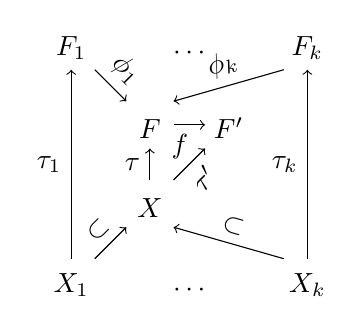
\begin{tikzpicture}
                \node [above] at (0,0) {$X_{1}$};
                \node [above] at (3,0) {$X_{k}$};
                \node [above] at (0,3) {$F_{1}$};
                \node [above] at (3,3) {$F_{k}$};
                \node [above] at (1,1) {$X$};
                \node [above] at (1,2) {$F$};
                \node [above] at (2,2) {$F'$};
                \node [above] at (1.5,0) {$\cdots$};
                \node [above] at (1.5,3) {$\cdots$};
                \draw [->] (0,0.6)-- node [left, pos=0.5] {$\tau_{1}$} (0,3);
                \draw [->] (3,0.6)-- node [left, pos=0.5] {$\tau_{k}$} (3,3);
                \draw [->] (0.3,0.6)-- node [above, pos=0.5, sloped] {$\subset$} (0.7,1);
                \draw [->] (1.3,1.6)-- node [below, pos=0.5, sloped] {$\tau'$} (1.7,2);
                \draw [->] (0.3,3)-- node [above, pos=0.5, sloped] {$\phi_{1}$} (0.7,2.6);
                \draw [->] (2.7,0.6)-- node [above, pos=0.5, sloped] {$\subset$} (1.3,1);
                \draw [->] (2.7,3)-- node [above, pos=0.5, sloped] {$\phi_{k}$} (1.3,2.6);
                \draw [->] (1,1.6)-- node [left, pos=0.5] {$\tau$} (1,2);
                \draw [->] (1.3,2.3)-- node [below, pos=0.2] {$f$} (1.7,2.3);
            \end{tikzpicture}
        \end{figure}
        \item For any $A$ with $f:X\to A$. Let $A=B\oplus C$ with $B=\{1_{R}a|a\in A\}$, $C=\{a\in A|1_{R}a=0\}$. So that $f(t)=b+c$ with $b\in B$, $c\in C$. Define $\bar{f}:R\oplus \mathbf{Z}\to A$ as $\bar{f}:(r,m)\mapsto rb+mc$. $f\tau(t)=b+c=f(t)\Rightarrow \bar{f}\tau=f$. $R\oplus \mathbf{Z}$ is free on $X$.
        \item If $R$ has indentity. Divide $X$ intoo singletons $\{x\}$. From (b), we have free module $F_{x}$ free on $\{x\}$. From (a), we have $\sum\limits_{x\in X}$ free on $X=\bigcup\limits_{x\in X}\{x\}$. If $R$ has no indentity. From Theorem III.1.10, we can embed $R$ into a ring $S$ with indentity. $S$ is an $R$-module. $\forall \{x\}\subset X$, $\tau(x)=1_{S}$ and for any $f:\{x\}\to A$ given by $f:x\mapsto a$. From \textbf{Exercise 4.1.18}, there exists unique homomorphism $\bar{f}:S\to A$, such that $f(1_{S})=a$. So $S$ is a free on $\{x\}$, thus $\sum\limits_{x\in X}S$ is free on $X$.
    \end{enumerate}
\end{answer}

$$ $$

\begin{ex}
    Let $R$ be any ring (possibly without indentity) and $F$ a free $R$-module on the set $X$, with $\tau X:\to F$, as in \textbf{Exercise 4.2.2}. Show that $\tau(X)$ is a set of generators of the $R$-module $F$.
\end{ex}

\begin{answer}
    Let $G$ be the submodule of $F$ generated by $\tau(X)$. $F$ is free on $X$ so that there exists unique $\varphi:F\to G$ with $\tau=\varphi\tau$. $\subset$ is the inclusion map, $\subset:G\to F$. $\subset\varphi=1_{F}\Rightarrow \varphi=1_{F}$.

    \begin{figure}[H]\centering
        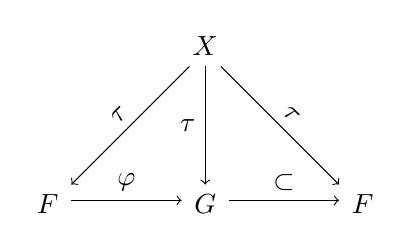
\begin{tikzpicture}
        \node [below] at (0,1) {$F$};
        \node [below] at (2,1) {$G$};
        \node [below] at (4,1) {$F$};
        \node [below] at (2,3) {$X$};
        \draw [->] (0.3,0.8)-- node [above, pos=0.5] {$\varphi$} (1.7,0.8);
        \draw [->] (2.3,0.8)-- node [above, pos=0.5] {$\subset$} (3.7,0.8);
        \draw [<-] (2,1)-- node [left, pos=0.5] {$\tau$} (2,2.5);
        \draw [<-] (0.3,1)-- node [above, pos=0.5, sloped] {$\tau$} (1.8,2.5);
        \draw [<-] (3.7,1)-- node [above, pos=0.5, sloped] {$\tau$} (2.2,2.5);
        \end{tikzpicture}
    \end{figure}
\end{answer}

$$ $$

\begin{ex}
    Let $R$ be a principal ideal domain, $A$ a unitary left $R$-module, and $p\in R$ a prime (= irreducible). Let $pA=\{pa|a\in A\}$ and $A[p]=\{a\in A|pa=0\}$.
    \begin{enumerate}[(a)]
        \item $R/(p)$ is a field.
        \item $pA$ and $A[p]$ are submodules of $A$.
        \item $A /pA$ is a vector space over $R /(p)$, with $(r+(p))(a+pA)=ra+pA$.
        \item $A[p]$ is a vector space over $R /(p)$, with $(r+(p))a=ra$.
    \end{enumerate}
\end{ex}

\begin{answer}
    \begin{enumerate}[(a)]
        \item $(p)$ is a prime ideal so $p$ is irreducible. $(p)$ is maximal. So $R /(p)$ is a field.
        \item $\forall a_{1},a_{2}\in pA$ and $r_{1},r_{2}\in R$, $a_{1}=pa_{1}'$, $a_{2}=pa_{2}'$, so \[r_{1}a_{1}+r_{2}a_{2}=r_{1}pa_{1}'+r_{2}pa_{2}'=p(r_{1}a_{1}'+r_{2}a_{2}')\in pA\] $pA$ is a submodule of $A$.
        
        $\forall a_{1},a_{2}\in A[p]$ and $r_{1},r_{2}\in R$, $pa_{1}=pa_{2}=0$ so \[p(r_{1}a_{1}+r_{2}a_{2})r_{1}pa_{1}+r_{2}pa_{2}=0\] $r_{1}a_{1}+r_{2}a_{2}\in A[p]$. $A[p]$ is a submodule of $A$.
        \item For any $a_{1}+pA, a_{2}+pA\in A /pA$ and $r_{1}+(p), r_{2}+(p)\in R /(p)$,\[(r_{1}+(p))(a_{1}+a_{2}+pA)=r_{1}a_{1}+r_{1}a_{2}pA=(r_{1}a_{1}+pA)+(r_{1}a_{2}+pA)\]\[(r_{1}+r_{2}+(p))(a_{1}+pA)=(r_{1}+r_{2})a_{1}+pA=(r_{1}a_{1}+pA)+(r_{2}a_{1}+pA)\]\[(r_{1}+(p))(r_{2}a_{1}+pA)=r_{1}r_{2}a_{1}+pA=(r_{1}r_{2}+(p))(a_{1}+pA)\] So $A /pA$ is an $R /(p)$-vector space.
        \item For any $a_{1},a_{2}\in A[p]$, $r_{1}+(p), r_{2}+(p)\in R /(p)$.\[(r_{1}+(p))(a_{1}+a_{2})=(r_{1}a_{1}+r_{1}a_{2})\in A[p]\]\[(r_{1}+(p))(r_{2}a_{1})=r_{1}r_{2}a_{1}=(r_{1}r_{2}+(p))a_{1}\]\[(r_{1}+r_{2}+(p))a_{1}=r_{1}a_{1}+r_{2}a_{2}\in A[p]\] $A[p]$ is an $R /(p)$-vector space. 
    \end{enumerate}
\end{answer}

$$ $$

\begin{ex}
    Let $V$ be a vector space over a division ring $D$ and $S$ the set of all subspaces of $V$, partiallly ordered by set theoretic inclusion.
    \begin{enumerate}[(a)]
        \item $S$ is a complete lattice.
        \item $S$ is a complemented lattice; that is, for each $V_{1}\in S$ there exists $V_{2}\in S$ such that $V=V_{1}+V_{2}$ and $V_{1}\cap V_{2}=0$, so that $V=V_{1}\oplus V_{2}$.
        \item $S$ is modular lattice; that is, if $V_{1}, V_{2}, V_{3}\in S$ and $V_{3}\subset V_{1}$, then \[V_{1}\cap (V_{2}+V_{3})=(V_{1}\cap V_{2})+V_{3}\]
    \end{enumerate}
\end{ex}

\begin{answer}
    \begin{enumerate}[(a)]
        \item Suppose there exists vector space $A$ satisfies that $V_{1}\subset A$, $V_{2}\subset A$. $\forall v_{1}\in V_{1}$, $v_{2}\in V_{2}$, $v_{1}+v_{2}\in A\Rightarrow V_{1}+V_{2}\subset A$. $V_{1}+V_{2}$ is the l.u.b. Similarly g.l.b is well-defined. For any subset $S'$ of $S$, $\sum\limits_{V\in S'}V$ is the l.u.b. $\bigcap\limits_{V\in S'}$ is the g.l.b. so $S$ is a complete lattice.
        \item Assume $B_{1}$ is the basis of $V_{1}$. $B_{1}$ can be extended into $B$, the basis of $V$. Take $V_{2}=\left\langle B\backslash B_{1}\right\rangle$, then $V_{1}\cap V_{2}=\varnothing
        $. For any $v\in V$, $v=\alpha_{1}w_{1}+\cdots+\alpha_{k}w_{k}+\alpha_{k+1}w_{k+1}+\cdots+\alpha_{n}w_{n}$ with $B_{1}=\{w_{1},\dots, w_{k}\}$. Then $v=v_{1}+v_{2}$, where $v_{1}=\alpha_{1}w_{1}+\cdots+\alpha_{k}w_{k}$, $v_{2}=\alpha_{k+1}w_{k+1}+\cdots+\alpha_{n}w_{n}$.
        \item For any $v_{2}+v_{3}\in (V_{2}+V_{3})\cap V_{1}$, $V_{3}\subset V_{1}$ so $v_{3}\in V_{1}$, $v_{2}\in V_{1}$. Thus $V_{1}\cap (V_{2}+V_{3})\subset V_{1}\cap V_{2}+V_{3}$.
        
        For any $v_{1}+v_{3}\in V_{1}\cap V_{2}+V_{3}$ with $v_{1}\in V_{2}$. $v_{1}+v_{3}\in V_{1}$ and $v_{1}+v_{3}\in V_{3}+V_{3}$. Thus $(V_{1}\cap V_{2})+V_{3}\subset V_{1}\cap (V_{2}+V_{3})$. $V_{1}\cap (V_{2}+V_{3})=(V_{1}\cap V_{2})+V_{3}$.
    \end{enumerate}
\end{answer}

$$ $$

\begin{ex}
    Let $\mathbf{R}$ and $\mathbf{C}$ be the fields of real and complex numbers respetively.
    \begin{enumerate}[(a)]
        \item $\mathrm{dim}_{\mathbf{R}}\mathbf{C}$ and $\mathrm{dim}_{\mathbf{R}}\mathbf{R}=1$.
        \item There is no field $K$ such that $\mathbf{R}\subset K\subset\mathbf{C}$.
    \end{enumerate}
\end{ex}

\begin{answer}
    \begin{enumerate}[(a)]
        \item It's not difficult to show $\{1\}$ is the basis of $\mathbf{R}$ and $\{1,i\}$ is the basis $B$ of $\mathbf{C}$. So $\dim_{\mathbf{R}}\mathbf{C}=2$, $\dim_{\mathbf{R}}\mathrm{R}=1$.
        \item Suppose not. $\mathbf{R}\subset K$ so $K$ is a vector space over $\mathbf{R}$. $\{1\}$ can be extended into $B$, a basis of $K$, $B$ can be extended into $\{1,i\}$ of $\mathbf{C}$. However, this is impossible. There's no such $K$ exists.
    \end{enumerate}
\end{answer}

$$ $$

\begin{ex}
    If $G$ is a nontrivial group that is not cyclic of order 2, then $G$ has a nonidentity automorphism.
\end{ex}

$$ $$

\begin{ex}
    If $V$ is a finite dimensional vector space and $V^{m}$ is the vector space\[V\oplus V\oplus\cdots\oplus V \,(m \text{ summands})\] then for each $m\geq 1$, $V^{m}$ is finite dimensional and $\mathrm{dim} V^{m}=m(\mathrm{dim}V)$.
\end{ex}

\begin{answer}
    $\bigoplus V$ is a $V$-module on $V$. We only need to check $\dim(V\oplus W)=\dim V+\dim W$. $\dim V+\dim W=\dim(V\cap W)+\dim (V+W)$. Since $V+W=V\oplus W$, $V\cap W$ is $0$. So $\dim V+\dim W=\dim(V\oplus W)$.
\end{answer}

$$ $$

\begin{ex}
    If $F_{1}$ and $F_{2}$ are free modules over a ring with the invariant dimension property, then $\mathrm{rank}(F_{1}\oplus F_{2})=\mathrm{rank}F_{1}+\mathrm{rank}F_{2}$.
\end{ex}

\begin{answer}
    Trivial since Corollary IV 2.14 is also true for a ring with invariant dimension property. 
\end{answer}

$$ $$

\begin{ex}
    Let $R$ be a ring with no zero divisors such that for all $r,s\in R$ there exists $a,b\in R$, not both zero, with $ar+bs=0$.
    \begin{enumerate}[(a)]
        \item If $R=K\oplus L$, then $K=0$ or $L=0$.
        \item If $R$ has an identity, then $R$ has the invariant dimension property.
    \end{enumerate}
\end{ex}

\begin{answer}
    \begin{enumerate}[(a)]
        \item If $K,L\neq 0$ and $l\in L$, for some $k\in K$ and $l\in L$, $\exists a,b\in R$ with $ak+bl=0$, so $K\cap L\neq 0$. $K+L$ can't be the direct sum.
    \end{enumerate}
\end{answer}

$$ $$

\begin{ex}
    Let $F$ be a free module of infinite rank $\alpha$ over a ring $R$ that has the invariant dimension property. For each cardinal $\beta$ such that $0\leq \beta\leq \alpha$, $F$ has infinitely many proper free submodules of rank $\beta$.
\end{ex}

$$ $$

\begin{ex}
    If $F$ is a free module ober a ring with indentity such that $F$ has a basis of finite cardinality $n\geq 1$ and another basis of cardinality $n+1$, then $F$ has a basis of cardinality $m$ for every $m\geq n$($m\in \mathbf{N}^{*}$).
\end{ex}

$$ $$

\begin{ex}
    Let $K$ be a ring with identity and $F$ a free $K$-module with an infinite demumerable basis $\{e_{1},e_{2},\dots\}$. Then $R=\mathrm{Hom}_{K}(F,F)$ is a ring by \textbf{Exercise 4.1.7}. If $n$ is any positive integer, then the free left $R$-module $R$ has a basis of $n$ elementsl that is,  as an $R$-module, $R\cong R\oplus\cdots\oplus R$ for any finite number of summands.
\end{ex}

\begin{answer}
    We prove for any $m\in \mathbf{N}$, we have $R\cong \sum\limits_{i=1}^{m}R$. Consider $B=\{f_{1}, f_{2}, \dot, f_{m}\}$, where $f_{i}:e_{km+i}\mapsto e_{k}$ and $f_{i}:e_{km+j}\mapsto 0$, $j\in \{1,2,\dots,m\}$, $j\neq i$. We show that $B$ is linearly independent and $R<\left\langle B\right\rangle$. Consider $f=\alpha_{1}f_{1}+\cdots+\alpha_{m}f_{m}$. Consider $f=0$, $f(e_{km+i})=\alpha_{i}f_{i}(e_{km+i})=\alpha_{i}e_{k}=0$ so $\alpha_{i}=0$ for all $i$, $B$ is linearly independent. For any $g\in R$, we first show that $g$ is uniquely determined by $g(\{e_{1},e_{2},\dots\})$. For any $x\in F$, WLOG, assume $x=\beta_{1}e_{1}+\beta_{2}e_{2}+\cdots+\beta_{k}e_{k}$ for some $e_{i}$. Then $g(x)=\beta_{1}g(e_{1})+\beta_{2}g(e_{2})+\cdots+\beta_{k}g(e_{k})$ is determined by $g(e_{1}), g(e_{2}),\dots, g(e_{k})\in g(\{e_{1},e_{2},\dots\})$. Then take $g_{i}$ as $g_{i}:e_{k}\mapsto g(e_{km+i})$. $g'=g_{1}f_{1}+\cdots+g_{m}f_{m}$. $g'(e_{k})=g(e_{k})$ for any $k$. Thus $g'=g$, $g\in \left\langle B\right\rangle$. $R\cong \bigoplus\limits_{f_{i}\in B}Rf_{i}$.
\end{answer}

$$ $$

\begin{ex}
    Let $f:V\to V'$ be a linear transformation of finite dimensional vector space $V$ and $V'$ such that $\mathrm{dim}V=\mathrm{dim}V'$. Then the following conditions are equivalent: (i) $f$ is an isomorphism; (ii) $f$ is an epimorphism $f$ is a monomorphism.
\end{ex}

\begin{answer}
    We only need to check (ii) and (iii) are equivalent.

    (ii)$\Rightarrow$(iii): Consider a basis $B'$ of $V'$. $B'=\{f(e_{1},f(e_{2}),\dots, f(e_{n}))\}$, take $B=\{e_{1},e_{2},\dots, e_{n}\}$. It's not difficult to prove $B$ is linearly independent. $\left| B \right|=\left| B' \right| =\dim V\Rightarrow \left\langle B\right\rangle=V$. For any $x,y\in V$, $x=\alpha_{1}e_{1}+\cdots+\alpha_{n}e_{n}$, $y=\beta_{1}e_{1}+\cdots+\beta_{n}e_{n}$, $f(x)=f(y)\Rightarrow (\alpha_{1}-\beta_{1})f(e_{1})+\cdots+(\alpha_{n}-\beta_{n})f(e_{n})=0$. $B'$ is linearly independent hence $\alpha_{i}=\beta_{i}$, $i=1,\dots$, which means $x=y$, $f$ is monomorphism.

    (iii)$\Rightarrow$(ii): Consider a basis $B$ of $V$. Similarly, we can prove $B'=f(B)$ is a basis of $V'$ since $f$ is monomorphism. $V'=\left\langle f(B)\right\rangle=f(\left\langle B\right\rangle)$. $f$ is epimorphism.
\end{answer}

$$ $$

\begin{ex}
    Let $R$ be a ring with identity. Show that $R$ is not a free module on any set in the category of all $R$-modules.
\end{ex}

\begin{answer}
    Consider a nonzero abelian group $A$ with $ra=0$ for all $r\in R$ and $a\in A$. $A$ is an $R$-module. Suppose $R$ is free on $X$ with $\tau:X\to R$, take any $f:X\to A$, we have $\bar{f}:R\to A$ such that $\bar{f}\tau=f$. However, $\bar{f}:R\to A$ must be the 0 map. That's contradictory!
\end{answer}